\chapter*{Metodyka badań}

\section*{Wprowadzenie do metodyki badań}

Niniejszy rozdział poświęcony jest metodyce badań, mającej na celu zbadanie wpływu tła na klasyfikację obrazów zwierząt 
przy użyciu zaawansowanych modeli głębokiego uczenia, takich jak ResNet i ConvNeXt. Badania te koncentrują się na 
analizie wyników klasyfikacji przed i po modyfikacjach tła z zastosowaniem różnych metryk oceny jakości, co pozwoli na 
zrozumienie, w jakim stopniu tło wpływa na wydajność modeli klasyfikacyjnych oraz jakie techniki mogą być stosowane do 
minimalizacji negatywnego wpływu tła. W pierwszej części rozdziału zostaną omówione narzędzia i oprogramowanie użyte do 
badań, konfiguracja sprzętowa i programowa, a także biblioteki i frameworki niezbędne do realizacji eksperymentów. 
Następnie przedstawione zostaną wybrane modele klasyfikacyjne, ResNet i ConvNeXt, wraz z uzasadnieniem ich wyboru oraz 
krótkim opisem ich architektur i specyfikacji. Kolejna sekcja skupi się na metrykach oceny jakości, z wyjaśnieniem, 
dlaczego właśnie te miary zostały wybrane oraz jak będą interpretowane wyniki. Opisany zostanie również zbiór danych 
wykorzystany w badaniach, jego źródło, struktura, etykiety oraz sposób przygotowania i przetwarzania danych przed 
użyciem w modelach. Kluczowym elementem rozdziału będzie szczegółowy plan przeprowadzenia badań, obejmujący wszystkie 
etapy, od segmentacji obrazów i usunięcia tła, poprzez modyfikację tła, aż po ocenę wyników modeli przed i po 
modyfikacjach. Całość zakończy krótkie podsumowanie metodyki badań, podkreślające główne kroki i decyzje podjęte w celu 
realizacji badań, co umożliwi systematyczną analizę wpływu tła na wyniki klasyfikacji obrazów oraz identyfikację 
najlepszych praktyk i metod poprawiających wydajność modeli klasyfikacyjnych.

\section*{Przygotowanie środowiska}

Przygotowanie odpowiedniego środowiska badawczego jest kluczowym krokiem w realizacji każdego projektu opartego na 
analizie danych i głębokim uczeniu. W niniejszych badaniach, całość prac została przeprowadzona w języku Python, który 
jest powszechnie stosowany w dziedzinie przetwarzania obrazów i uczenia maszynowego dzięki bogatemu ekosystemowi 
bibliotek i narzędzi wspomagających te procesy.

Do realizacji projektu użyto następujących bibliotek: numpy, pandas, scikit-learn, PIL, matplotlib, seaborn oraz torch. 
Biblioteka numpy została wykorzystana do obsługi operacji numerycznych i manipulacji tablicami, biblioteka pandas służyła 
do manipulacji i analizy danych strukturalnych, takich jak tablice. Scikit-learn był wykorzystywany przy obliczeniach 
metryk i ocenie jakości modeli, a PIL (Python Imaging Library) umożliwiła manipulację obrazami. Biblioteki matplotlib i 
seaborn posłużyły do wizualizacji danych i wyników analiz, co pozwoliło na lepsze zrozumienie uzyskanych rezultatów oraz 
prezentację wyników w formie graficznej.

Kluczowym elementem projektu były zaawansowane modele głębokiego uczenia: ResNet, ConvNeXt oraz DeepLabv3. Modele te 
zostały zaimportowane z biblioteki torchvision, która jest częścią ekosystemu PyTorch. Torchvision dostarcza łatwy 
dostępu do najnowocześniejszych modeli pretrenowanych na dużych zbiorach danych, co umożliwia efektywne przeprowadzanie 
eksperymentów bez konieczności trenowania modeli od podstaw.

Dodatkowo, do analizowania wyników i prowadzenia interaktywnej pracy z kodem, używany był Jupyter Notebook. Jupyter 
Notebook jest wszechstronnym narzędziem, które umożliwia tworzenie i udostępnianie dokumentów zawierających kod, 
równania, wizualizacje oraz tekst. Jego zastosowanie pozwoliło na przejrzyste prezentowanie procesu badawczego, 
testowanie i modyfikowanie kodu w czasie rzeczywistym oraz dokumentowanie każdego kroku analizy.

Całe środowisko badawcze zostało skonfigurowane na lokalnym komputerze wyposażonym w GPU. Korzystanie z GPU było kluczowe
dla efektywnego przeprowadzania eksperymentów, zwłaszcza w kontekście obliczeniowo intensywnych operacji związanych z 
przetwarzaniem obrazów. W ramach projektu zastosowano system kontroli wersji GIT, a cały kod źródłowy oraz wyniki 
analiz zostały zapisane i wersjonowane na platformie GitHub. Użycie GIT umożliwiło efektywne śledzenie zmian w kodzie, 
co pozwoliło na łatwe zarządzanie i kontrolowanie wersji poszczególnych plików oraz eksperymentów. Dzięki temu każdy 
etap projektu był dokładnie dokumentowany, co ułatwiało powrót do wcześniejszych wersji kodu w razie potrzeby oraz 
analizę postępów prac. Ponadto, platforma GitHub zapewniła bezpieczne i zorganizowane przechowywanie kodu.

Odpowiednie przygotowanie środowiska z użyciem wymienionych narzędzi i bibliotek było fundamentem dla 
przeprowadzenia skutecznych i efektywnych badań nad wpływem tła na klasyfikację obrazów.

\section*{Wybrane modele}

W niniejszym projekcie zastosowano trzy zaawansowane modele głębokiego uczenia: ResNet, ConvNeXt oraz DeepLabv3. 
Każdy z tych modeli został wybrany ze względu na swoje unikalne właściwości i zdolności do realizacji określonych zadań. 
DeepLabv3 służył jako uniwersalny model do segmentacji, pozwalający na precyzyjne wyodrębnienie obiektów z tła. 
Modele ResNet i ConvNeXt, o różnych architekturach i z różnymi stopniami zaawansowania technologicznego, zostały 
wykorzystane do klasyfikacji obrazów. ResNet, będący starszym modelem, oraz ConvNeXt, reprezentujący nowsze podejście, 
zostały wybrane w celu porównania i analizy ich wydajności w kontekście zmodyfikowanych warunków tła. Wykorzystanie 
gotowych, pretrenowanych modeli umożliwiło skupienie się na głównej części badania, jaką jest wpływ tła na klasyfikację 
obrazów, zamiast na długotrwałym procesie trenowania modeli od podstaw.

\subsection*{ResNet}

ResNet (Residual Network) został zaproponowany w 2015 roku i szybko stał się jednym z najważniejszych modeli w 
dziedzinie głębokiego uczenia. Główną innowacją ResNet jest wprowadzenie residual learning poprzez zastosowanie 
skrótowych połączeń (skip connections). Pozwala to na efektywne trenowanie bardzo głębokich sieci, nawet o setkach 
warstw, rozwiązując problem zanikania gradientu.

W tradycyjnych sieciach neuronowych, gdy liczba warstw wzrasta, problem zanikania gradientu staje się bardziej wyraźny, 
co utrudnia efektywne trenowanie modeli. ResNet adresuje ten problem poprzez wprowadzenie bezpośrednich połączeń 
skrótowych, które umożliwiają przepływ gradientu bezpośrednio przez sieć, omijając kilka warstw pośrednich.

Podstawowym elementem budulcowym ResNet jest blok residual, który może być opisany równaniem:

\begin{equation}
    y = F(x, \{W_i\}) + x
\end{equation}

gdzie \( y \) to wyjście bloku, \( x \) to wejście, a \( F(x, \{W_i\}) \) to funkcja reprezentująca operacje 
konwolucyjne na wejściu \( x \) z zestawem wag \( \{W_i\} \).

Bloki residual składają się zazwyczaj z dwóch lub trzech warstw konwolucyjnych z dodatkowymi połączeniami skrótowymi, 
które dodają wejście \( x \) do wyjścia \( F(x, \{W_i\}) \). To proste, ale skuteczne podejście pozwala na trenowanie 
bardzo głębokich sieci, które byłyby trudne do nauczenia przy użyciu tradycyjnych metod.

ResNet został wybrany do tego projektu ze względu na swoją zdolność do efektywnego radzenia sobie z bardzo głębokimi 
sieciami oraz udowodnioną skuteczność w wielu zadaniach klasyfikacyjnych. 

Konkretnym modelem użytym w przeprowadzonych badaniach
jest ResNet50. Architektura ResNet50 jest podzielona na cztery główne części: warstwy konwolucyjne, blok tożsamościowy, 
blok konwolucyjny oraz warstwy całkowicie połączone. Schemat architektury tego modelu można zobaczyć na Rys. \ref*{rys:resnet}

Warstwy konwolucyjne w ResNet50 składają się z kilku warstw konwolucyjnych, po których następuje normalizacja wsadowa 
(batch normalization) oraz aktywacja ReLU. Warstwy te są odpowiedzialne za ekstrakcję cech z obrazu wejściowego, takich jak 
krawędzie, tekstury i kształty. Następnie warstwy konwolucyjne są uzupełnione warstwami maksymalnego pooling (max pooling), 
które redukują przestrzenne wymiary map cech, jednocześnie zachowując najważniejsze cechy.

Blok tożsamościowy (identity block) i blok konwolucyjny (convolutional block) są kluczowymi elementami budulcowymi ResNet50. 
Blok tożsamościowy jest prostym blokiem, który przekazuje wejście przez szereg warstw konwolucyjnych i dodaje wejście z 
powrotem do wyjścia. Pozwala to sieci uczyć się funkcji resztkowych, które mapują wejście na pożądane wyjście. Blok konwolucyjny 
jest podobny do bloku tożsamościowego, ale z dodatkiem warstwy konwolucyjnej 1x1, która jest używana do redukcji liczby filtrów 
przed warstwą konwolucyjną 3x3.

Ostatnią częścią ResNet50 są warstwy całkowicie połączone (fully connected layers). Warstwy te są odpowiedzialne za dokonanie 
ostatecznej klasyfikacji. Wyjście z ostatniej warstwy całkowicie połączonej jest przekazywane do funkcji aktywacji softmax, aby 
uzyskać ostateczne prawdopodobieństwa klas.

\begin{figure}
	\centering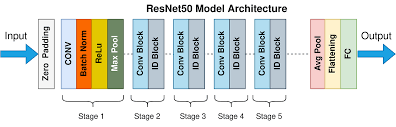
\includegraphics[width=.9\textwidth]{img/resnet.png}
	\caption{Schemat architektury modelu ResNet50}  \label{rys:resnet}
\end{figure}

\subsection*{ConvNeXt}

ConvNeXt to nowoczesna architektura CNN, która została opracowana w celu integracji najlepszych praktyk z konwolucyjnych 
sieci neuronowych i nowoczesnych technik pochodzących od transformerów. ConvNeXt wykorzystuje bardziej złożone operacje 
konwolucyjne oraz zaawansowane techniki normalizacji i optymalizacji, co pozwala na osiąganie znakomitych wyników w 
różnych zadaniach klasyfikacji.

ConvNeXt został zaprojektowany z myślą o zastosowaniu najnowszych technik z dziedziny głębokiego uczenia, takich jak 
normalizacja warstw (Layer Normalization), mechanizmy uwagi (Attention Mechanisms) oraz bardziej złożone architektury 
warstw konwolucyjnych. W ConvNeXt zastosowano podejście polegające na udoskonaleniu tradycyjnych modułów konwolucyjnych 
poprzez dodanie elementów inspirowanych transformerami, co prowadzi do lepszej wydajności i efektywności obliczeniowej.

Podstawowym elementem ConvNeXt jest moduł konwolucyjny, który został zoptymalizowany w celu lepszego uchwycenia 
złożonych wzorców w danych. Architektura ConvNeXt łączy tradycyjne podejścia konwolucyjne z nowymi koncepcjami, co 
prowadzi do lepszej wydajności i efektywności obliczeniowej.

ConvNeXt został wybrany do tego projektu ze względu na swoje nowoczesne podejście i wysoką wydajność w klasyfikacji 
obrazów, co pozwala na dokładne porównanie z wcześniejszymi modelami, takimi jak ResNet.

\subsection*{DeepLabv3}

DeepLabv3 jest modelem segmentacji obrazów, który został opracowany przez zespół Google. Wykorzystuje on techniki 
takie jak atrous convolutions (dylatowane konwolucje) i Conditional Random Fields (CRFs), które pozwalają na dokładne 
modelowanie kontekstowych informacji na różnych skalach. DeepLabv3+ jest najnowszą wersją tej serii, która łączy atrous 
convolutions z modulem spatial pyramid pooling, co pozwala na uchwycenie bogatych informacji kontekstowych.

Podstawowym elementem DeepLabv3 jest zastosowanie atrous convolutions, które mogą być opisane równaniem:

\begin{equation}
y[i] = \sum_{k=1}^{K} x[i + r \cdot k] \cdot w[k]
\end{equation}

gdzie \( y[i] \) to wyjście konwolucji, \( x \) to wejście, \( w \) to zestaw wag, \( K \) to rozmiar filtra, a \( r \) 
to współczynnik dylatacji.

Dzięki zastosowaniu atrous convolutions, DeepLabv3 może uchwycić informacje na różnych skalach bez utraty 
rozdzielczości, co jest kluczowe dla dokładnej segmentacji. Dodatkowo, wykorzystanie spatial pyramid pooling pozwala na 
zbieranie informacji kontekstowych z całego obrazu, co poprawia dokładność segmentacji.

DeepLabv3 został wybrany ze względu na swoją zdolność do precyzyjnej segmentacji obrazów, co jest kluczowe dla 
wyodrębnienia obiektów z tła przed dalszą analizą i klasyfikacją.

\subsection*{Uzasadnienie wyboru modeli}

Wybór ResNet, ConvNeXt oraz DeepLabv3 opierał się na ich sprawdzonej skuteczności w swoich dziedzinach oraz zdolności 
do realizacji celów tego projektu. ResNet, jako starszy model, pozwala na ocenę wpływu tła na klasyfikację obrazów w 
kontekście bardziej tradycyjnych architektur. ConvNeXt, będący nowoczesnym modelem, reprezentuje najnowsze podejścia i 
innowacje w dziedzinie głębokiego uczenia, co pozwala na ocenę, jak nowe technologie radzą sobie z problemem tła. 
DeepLabv3, jako zaawansowany model segmentacji, umożliwia precyzyjne usunięcie tła, co jest kluczowe dla analiz 
prowadzonych w ramach tego projektu.

Wykorzystanie gotowych, pretrenowanych modeli pozwoliło skupić się na głównym celu badania – analizie wpływu tła na 
klasyfikację obrazów – bez konieczności poświęcania czasu na trenowanie modeli od podstaw. Dzięki temu możliwe było 
przeprowadzenie bardziej szczegółowych i kompleksowych badań w zakresie modyfikacji tła i jego wpływu na wydajność 
modeli klasyfikacyjnych.

\section*{Wybrane metryki}

W celu analizy wyników klasyfikacji przed i po modyfikacjach tła, zastosowano dwie kluczowe metryki, dokładności 
(accuracy) oraz pewności klasyfikacji (confidence scores). Analizowana będzie również macierz pomyłek w celu zbadania
najczęsciej mylących się klas, oraz zbdania jakie błędy zostały popełnione. Metryki te zostały wybrane ze względu na ich zdolność do 
dostarczania wartościowych informacji na temat wydajności modeli w różnych warunkach. W niniejszym rozdziale szczegółowo 
omówimy te metryki, przedstawimy odpowiednie wzory oraz wyjaśnimy, dlaczego zostały wybrane do analizy. Metryki będą 
analizowane całościowo, jak również osobno dla każdej klasy, dla każdej różnej modyfikacji tła oraz dla różnych 
percentyli wielkości obiektu na obrazie.

\subsection*{Dokładność (Accuracy)}

Dokładność jest jedną z najprostszych i najbardziej intuicyjnych metryk stosowanych do oceny jakości modeli 
klasyfikacyjnych. Definiuje się ją jako stosunek liczby poprawnie sklasyfikowanych przykładów do całkowitej liczby 
przykładów.

Wzór na dokładność jest następujący:

\begin{equation}
\text{Accuracy} = \frac{TP + TN}{TP + TN + FP + FN}
\end{equation}

gdzie:
\begin{itemize}
    \item TP (True Positives) - liczba prawdziwie pozytywnych przypadków,
    \item TN (True Negatives) - liczba prawdziwie negatywnych przypadków,
    \item FP (False Positives) - liczba fałszywie pozytywnych przypadków,
    \item FN (False Negatives) - liczba fałszywie negatywnych przypadków.
\end{itemize}

Dokładność została wybrana jako podstawowa metryka oceny modeli, ponieważ daje ogólny obraz wydajności modelu.

\subsection*{Pewność klasyfikacji (Confidence Scores)}

Pewność klasyfikacji (confidence scores) odnosi się do stopnia pewności modelu co do przypisania danego przykładu do 
określonej klasy. Jest to istotna metryka, ponieważ dostarcza dodatkowych informacji o tym, jak pewny jest model swoich 
predykcji. Wyższe wartości pewności oznaczają większe zaufanie modelu do swojej klasyfikacji.

Analiza pewności klasyfikacji pozwala na ocenę, jak model radzi sobie z przypadkami trudnymi do sklasyfikowania oraz 
czy zmiany tła wpływają na pewność predykcji.

\subsection*{Macierz pomyłek}

Macierz pomyłek (confusion matrix) jest narzędziem używanym do oceny wydajności modeli klasyfikacyjnych poprzez 
pokazanie, jak często poszczególne klasy są mylone z innymi. Macierz pomyłek przedstawia liczbę prawdziwie pozytywnych, 
prawdziwie negatywnych, fałszywie pozytywnych i fałszywie negatywnych klasyfikacji dla każdej klasy.

W przypadku klasyfikacji wieloklasowej, macierz pomyłek rozszerza się do macierzy n×n, gdzie n to liczba klas. 
Każda komórka Cij​ w macierzy pomyłek przedstawia liczbę przypadków należących do klasy i, które zostały 
sklasyfikowane jako klasa j.

Analiza macierzy pomyłek pozwala na identyfikację, które klasy są najczęściej mylone, co może dostarczyć cennych 
informacji na temat specyficznych wyzwań związanych z klasyfikacją w kontekście zmodyfikowanych teł.

\section*{Opis wykorzystanego zbioru danych}

W ramach niniejszego badania wykorzystano zbiór danych ImageNet1k, który jest jednym z najbardziej rozpoznawalnych i 
szeroko stosowanych zestawów danych w dziedzinie przetwarzania obrazów i głębokiego uczenia. ImageNet1k składa się z 
obrazów należących do 1000 różnych klas, co pozwala na wszechstronną ocenę wydajności modeli klasyfikacyjnych w 
różnorodnych scenariuszach.

\subsection*{Struktura zbioru danych}

Zbiór danych ImageNet1k jest podzielony na trzy części: treningową, walidacyjną oraz testową. Każda z tych części ma 
określoną liczbę obrazów na klasę, co umożliwia wszechstronne trenowanie, walidację i testowanie modeli klasyfikacyjnych.

\begin{itemize}
    \item \textbf{Zbiór treningowy:} Zawiera około 1300 obrazów na klasę, co daje szeroką bazę danych do nauki modeli. 
    Duża liczba obrazów na klasę pozwala na efektywne trenowanie głębokich sieci neuronowych, co prowadzi do lepszego 
    uchwycenia cech charakterystycznych dla każdej klasy.
    \item \textbf{Zbiór walidacyjny:} Składa się z 50 obrazów na klasę. Zbiór walidacyjny jest używany do monitorowania 
    wydajności modelu w trakcie treningu i do wczesnego wykrywania problemów takich jak nadmierne dopasowanie 
    (overfitting).
    \item \textbf{Zbiór testowy:} Zawiera 100 obrazów na klasę. Zbiór testowy służy do ostatecznej oceny wydajności 
    modeli po zakończeniu procesu treningu i walidacji.
\end{itemize}

\subsection*{Różnorodność obrazów}

Obrazy w zbiorze ImageNet1k charakteryzują się różnorodnością rozdzielczości oraz warunków, w jakich zostały wykonane. 
Oznacza to, że obrazy mogą przedstawiać obiekty w różnych skalach, oświetleniach, perspektywach i na różnych tłach. 
Taka różnorodność sprawia, że zbiór ImageNet1k doskonale odzwierciedla realistyczne warunki, z jakimi modele mogą się 
spotkać w praktycznych zastosowaniach. Dzięki temu, modele trenowane na tym zbiorze danych są bardziej uniwersalne i 
mają lepszą zdolność generalizacji. 

\subsection*{Popularność i znaczenie ImageNet1k}

ImageNet1k jest jednym z najczęściej używanych zestawów danych w badaniach nad głębokim uczeniem, co jest wynikiem 
jego dużej skali, różnorodności i realistycznego charakteru. Wiele przełomowych modeli, takich jak AlexNet, VGG, 
ResNet i Inception, zostało przetestowanych i zweryfikowanych przy użyciu tego zestawu danych. Popularność ImageNet1k 
sprawia, że wyniki uzyskane na tym zbiorze są łatwo porównywalne z wynikami innych badań, co umożliwia ocenę postępów i 
innowacji w dziedzinie przetwarzania obrazów.

Ze względu na ograniczoną dostępność klas w modelu segmentacyjnym DeepLabv3,
który był trenowany na innym zbiorze danych, do badań wybrano 10 klas zwierząt, które można skutecznie wysegmentować 
przy użyciu tego modelu. Wybór tych klas pozwolił na przeprowadzenie dokładnych analiz i eksperymentów przy zachowaniu 
rozsądnego czasu przetwarzania.


\section*{Plan badań}

Niniejszy rozdział opisuje szczegółowy plan badań, które zostały przeprowadzone w celu zbadania wpływu tła na 
klasyfikację obrazów zwierząt. Poniżej przedstawiono kroki podjęte w celu realizacji 
badań.

\subsection*{Przygotowanie środowiska pracy}

Pierwszym krokiem było przygotowanie odpowiedniego środowiska pracy. W tym celu skonfigurowano środowisko 
programistyczne, które obejmowało instalację niezbędnych bibliotek i narzędzi, takich jak numpy, pandas, scikit-learn, 
PIL, matplotlib, seaborn, torch oraz torchvision. Zastosowano również system kontroli wersji GIT do śledzenia zmian w 
kodzie i zarządzania wersjami projektu.

\subsection*{Wybranie modeli do segmentacji i klasyfikacji}

Do segmentacji obrazów wybrano model DeepLabv3, który jest zaawansowanym modelem segmentacji zdolnym do precyzyjnego 
wyodrębniania obiektów z tła. Do klasyfikacji obrazów wybrano dwa modele: ResNet, reprezentujący starszą generację 
modeli głębokiego uczenia, oraz ConvNeXt, będący nowszym i bardziej zaawansowanym modelem. Wybór tych modeli pozwolił 
na dokładne porównanie ich wydajności w kontekście różnych modyfikacji tła.

\subsection*{Wybranie klas zwierząt}

Ze względu na ograniczoną dostępność klas w modelu segmentacyjnym DeepLabv3, do badań wybrano 10 zróżnicowanych klas 
zwierząt. Wybrane klasy były takie, które można skutecznie wysegmentować przy użyciu tego modelu, co pozwoliło na 
przeprowadzenie dokładnych analiz i eksperymentów. Przykładowe zdjęcia dla każdej wybranej klasy można zaobserwować na Rys. \ref{rys:classes}

\begin{figure}
	\centering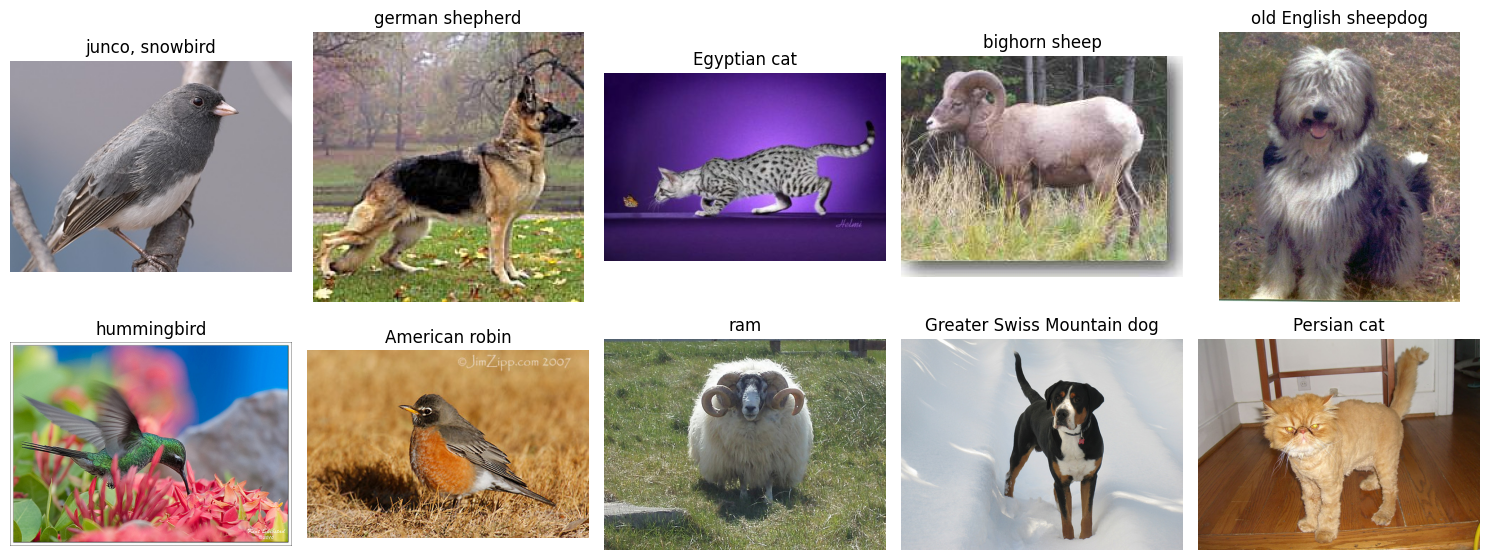
\includegraphics[width=.9\textwidth]{img/classes}
	\caption{Przykładowe oryginalne zdjęcia wybranych klas}  \label{rys:classes}
\end{figure}

\subsection*{Segmentacja obrazów}

Dla każdej z wybranych klas zwierząt wysegmentowano 1000 zdjęć za pomocą modelu DeepLabv3. Ponieważ na niektórych 
zdjęciach widniało więcej klas obiektów rozpoznawanych przez ten model, konieczne było zidentyfikowanie wartości grayscale dla pożądanej maski 
obiektu. W tym celu zastosowano skrypt analizujący najczęściej występującą wartość na przestrzeni wszystkich zdjęć 
dla danej klasy, co pozwoliło na dokładne wyodrębnienie obiektów. Maski zostały zapisane do dalszych analiz. Przykładowe uzyskane
maski można zaobserwować na Rys. \ref{rys:masks}

\begin{figure}
	\centering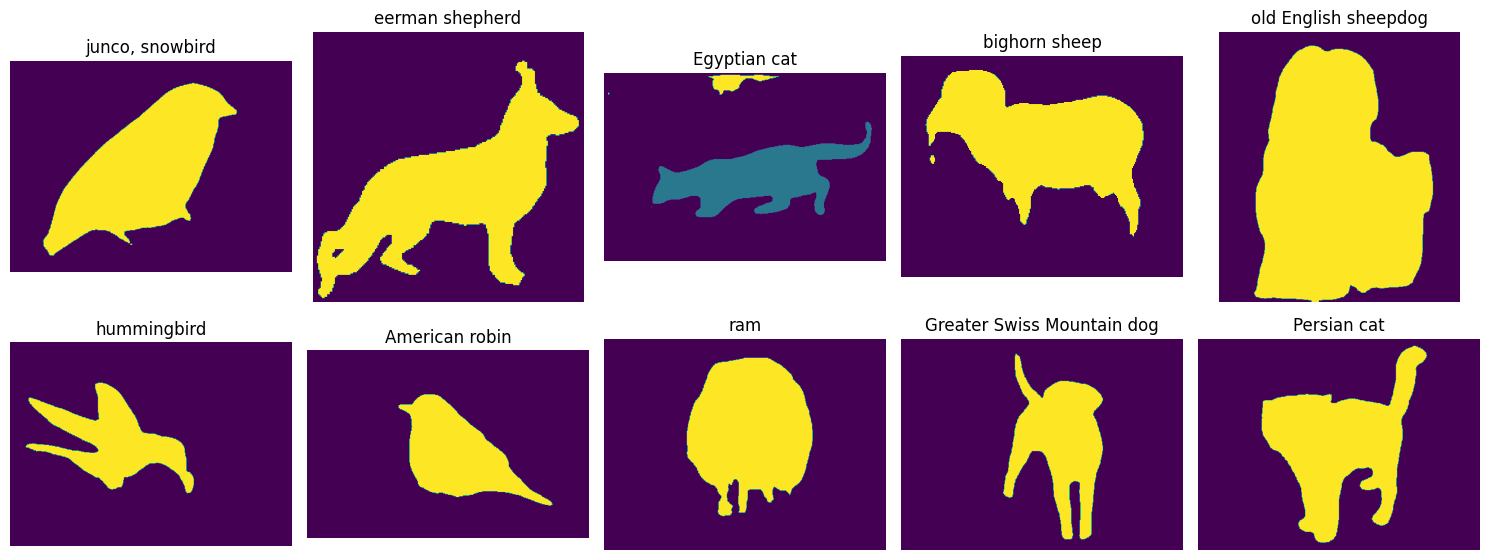
\includegraphics[width=.9\textwidth]{img/masks}
	\caption{Maski przykładowych wysegmentowanych obrazów}  \label{rys:masks}
\end{figure}

\subsection*{Przygotowanie zmodyfikowanych zbiorów zdjęć}

Dla każdej klasy zwierząt przygotowano różne zestawy zmodyfikowanych zdjęć:
\begin{itemize}
    \item \textbf{Zdjęcia z samym obiektem:} Usunięto tło za pomocą maski, pozostawiając czarne tło.
    \item \textbf{Zdjęcia z samym tłem:} Odwrotna modyfikacja do poprzedniej, pozostawiając samo tło bez obiektu.
    \item \textbf{Przeniesienie obiektu na różne scenerie:} Obiekty zostały przeniesione na różne tła, takie jak niebo, 
    wnętrze domu, pustynia, śnieg, woda, miasto, dżungla, góry.
    \item \textbf{Zastąpienie tła kolorem o niskim oraz wysokim kontraście do obiektu:} Dla każdej klasy zwierząt zbierano próbki kolorów. 
    Obrazy były wczytywane i konwertowane do tablicy NumPy, a następnie tworzono maskę, która ignorowała czarne piksele 
    (wartości RGB: 0, 0, 0), aby skupić się wyłącznie na rzeczywistych kolorach obiektów. Zebrane próbki kolorów były następnie 
    klasteryzowane za pomocą algorytmu KMeans z pięcioma klastrami, co pozwalało na wyodrębnienie pięciu dominujących kolorów dla 
    każdej klasy zwierząt. Dominujące kolory były normalizowane do skali 0-1, a następnie obliczana była ich średnia wartość, 
    uznawana za kolor o niskim kontraście. Odległości euklidesowe każdego koloru od średniej wartości były obliczane, a kolor 
    najbardziej oddalony od średniej był uznawany za kolor o wysokim kontraście. Ostatecznie, kolory były konwertowane z powrotem 
    na skalę 0-255 i zapisywane jako wartości RGB. 
\end{itemize}

Przykładowe zdjęcie, wraz z jego modyfikacjami można zobaczyć na Rys. \ref*{rys:modified}

\begin{figure}
	\centering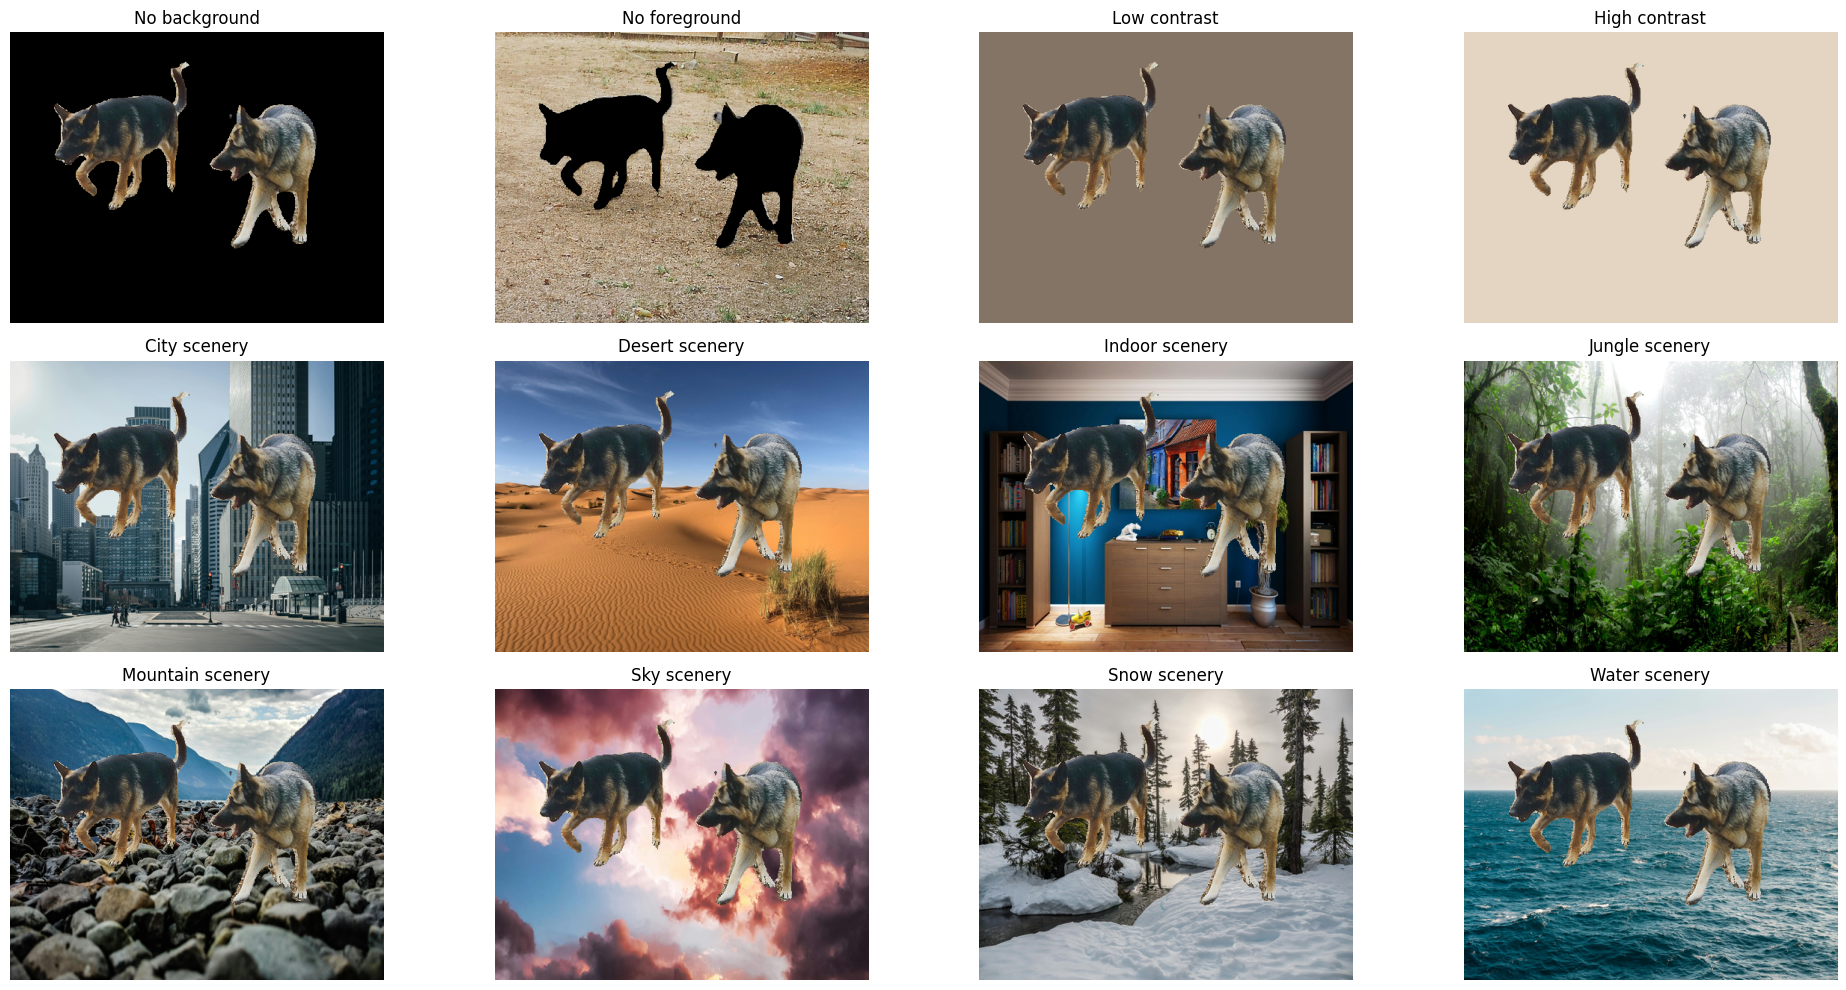
\includegraphics[width=.9\textwidth]{img/modified}
	\caption{Przykładowe zdjęcie poddane modyfikacją}  \label{rys:modified}
\end{figure}

\subsection*{Dokonanie predykcji na wybranych modelach}

Predykcje zostały przeprowadzone na wybranych modelach ResNet oraz ConvNeXt dla oryginalnych zdjęć oraz dla każdej 
modyfikacji tła. Wyniki predykcji, w tym klasyfikacje oraz pewność klasyfikacji (confidence scores), zostały zapisane w
plikach CSV.

\subsection*{Dodanie kategorii zdjęć pod względem procentu zajmowanego przez obiekt na zdjęciu}

Zbadanie stosunku wielkości obiektu do całego zdjęcia jest istotne w kontekście badania wpływu tła na klasyfikację, ponieważ 
może znacząco wpływać na wyniki modeli klasyfikacyjnych. Wielkość obiektu w stosunku do tła może determinować, jak łatwo model 
jest w stanie rozpoznać i sklasyfikować obiekt. Mniejsze obiekty mogą być trudniejsze do wykrycia i bardziej podatne na 
zakłócenia ze strony tła, podczas gdy większe obiekty mogą dominować obraz, co ułatwia ich klasyfikację. Analiza wpływu różnych 
procentyli wielkości obiektu pozwala na zrozumienie, w jakim stopniu tło oddziałuje na modele w zależności od proporcji obiektu 
na zdjęciu, co z kolei może prowadzić do bardziej efektywnych strategii przetwarzania i klasyfikacji obrazów w praktycznych 
zastosowaniach.

Dla każdego zdjęcia dodano kategorię pod względem procentu zajmowanego przez obiekt na zdjęciu. Przykładowe zdjęcia o różnych 
rozmiarach obiektów można zobaczyć na Rys. \ref*{rys:size_comp}

\begin{enumerate}
    \item \textbf{Obliczenie powierzchni obiektu:} Dla każdego obrazu obliczono liczbę pikseli zajmowanych przez obiekt.
    \item \textbf{Obliczenie powierzchni całkowitej obrazu:} Liczba pikseli całego obrazu.
    \item \textbf{Obliczenie procentu powierzchni zajmowanej przez obiekt:} Procent powierzchni zajmowanej przez obiekt obliczono za pomocą wzoru:
    \begin{equation}
    \text{Procent powierzchni zajmowanej przez obiekt} = \left( \frac{\text{Powierzchnia obiektu}}{\text{Powierzchnia całkowita obrazu}} \right) \times 100
    \end{equation}
    \item \textbf{Podział obiektów na percentyle:} Obrazy posortowano według procentu powierzchni zajmowanej przez obiekt i 
    podzielono na cztery grupy według wartości percentyli.
\end{enumerate}

\begin{figure}
	\centering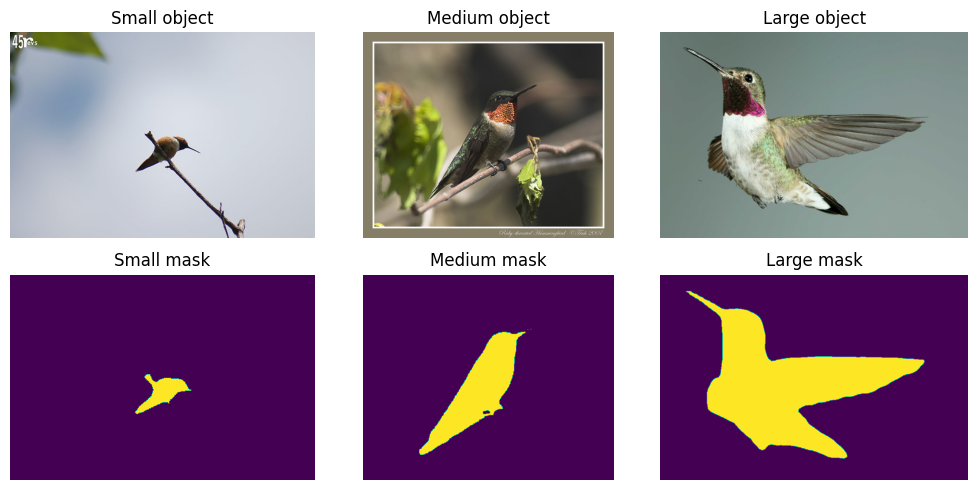
\includegraphics[width=.9\textwidth]{img/size_comp}
	\caption{Przykładowe zdjęcia o różnych rozmiarach obiektów dla klasy "hummingbird"}  \label{rys:size_comp}
\end{figure}

\subsection*{Analiza wyników}

Wyniki zostały poddane szczegółowej analizie w kilku aspektach:
\begin{itemize}
    \item \textbf{Analiza ogólna wyników:} Ogólna wydajność modeli na całym zbiorze danych.
    \item \textbf{Analiza pod kątem klasy:} Wydajność modeli dla każdej klasy zwierząt osobno.
    \item \textbf{Analiza pod kątem wielkości obiektu:} Wydajność modeli w zależności od wielkości obiektu na zdjęciu (cztery percentyle).
    \item \textbf{Porównanie modeli:} Porównanie wyników starszego modelu ResNet oraz nowszego ConvNeXt.
\end{itemize}

\subsection*{Wnioski i dalsze kierunki rozwoju}

Na podstawie przeprowadzonych analiz wyciągnięto wnioski dotyczące wpływu tła na wyniki klasyfikacji obrazów zwierząt. Ponadto zaproponowano dalsze kierunki rozwoju, mające na celu optymalizację modeli klasyfikacyjnych w kontekście zmieniających się warunków tła.

\subsection*{Podsumowanie}

Plan badań obejmował szczegółowe przygotowanie środowiska pracy, wybór odpowiednich modeli do segmentacji i klasyfikacji, segmentację obrazów, przygotowanie zmodyfikowanych zbiorów zdjęć oraz przeprowadzenie predykcji i analiz wyników. Dzięki systematycznemu podejściu możliwe było uzyskanie wartościowych wniosków na temat wpływu tła na wydajność modeli klasyfikacyjnych oraz identyfikacja obszarów wymagających dalszych badań i optymalizacji.
